\subsection{Target Geometry}\label{sec:targetgeom}
\begin{figure}
\centerline{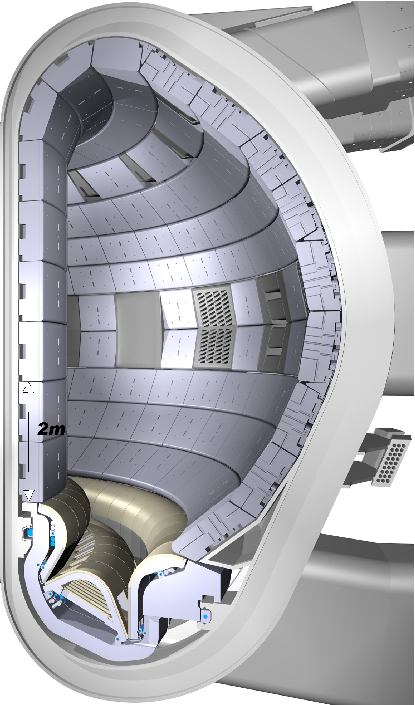
\includegraphics[width=8cm]{../png/iterfw}}
\caption{The complexity of the ITER first wall\label{fig:iterfw}}
\end{figure}
\begin{figure}
\centerline{
\includegraphics[width=6cm]{../png/jetdiveclose}
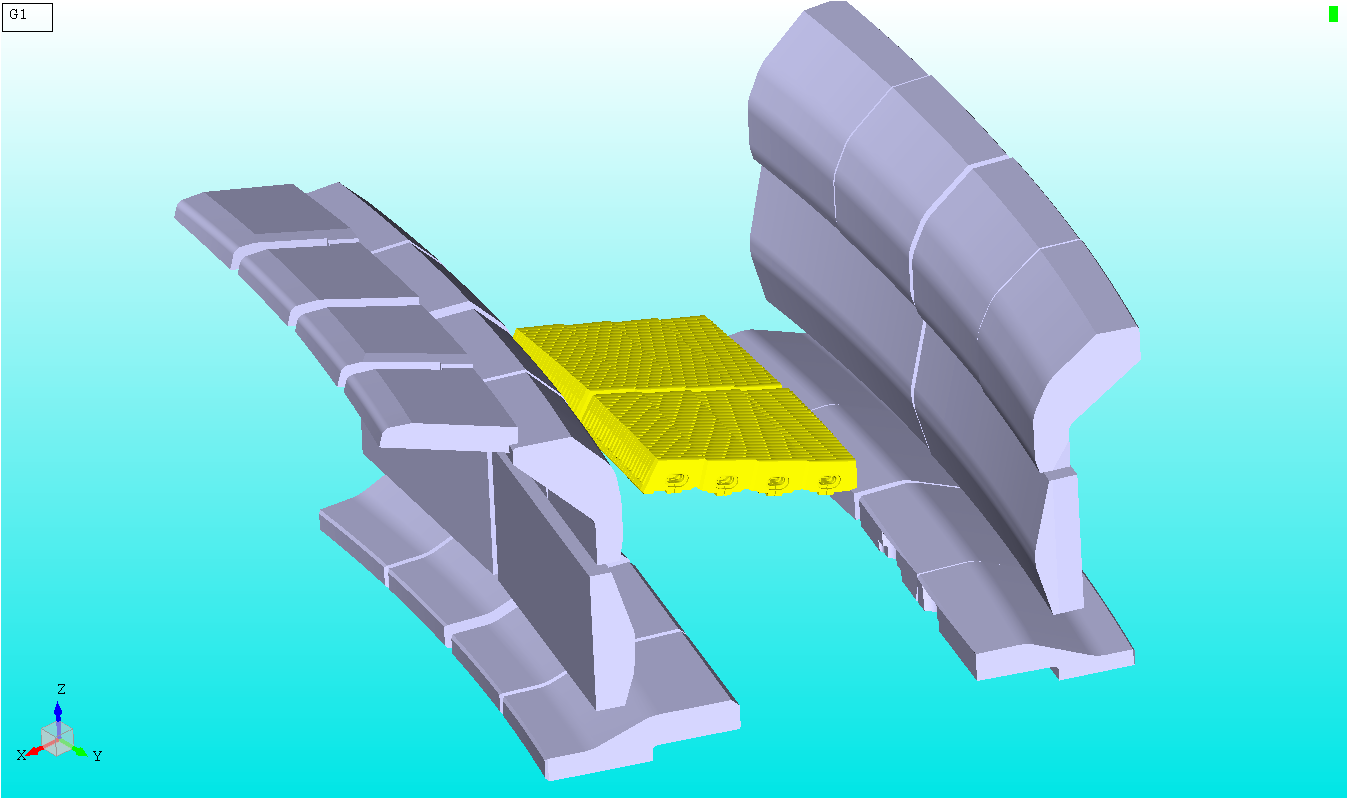
\includegraphics[width=6cm]{../png/pretty}}
\caption{Close-up of the JET divertor showing individual tiles (left) and
simplified CAD representation (right).\label{fig:jetdive}}
\end{figure}
\Fig{iterfw} indicates the complexity of the designed geometry of the
ITER tokamak interior, which \Fig{jetdive} indicates might be less than that of an actual device
after, in the JET case, incorporation of new divertor and other upgrades in the operational phase.
The ITER wall is covered with tiles, there are ducts entering from the right (shown
blanked off), grilles protecting antennas, and the divertor chamber at the bottom, with
exposed support structures in some designs. All these features may have to be 
dealt with by a SOL code. Further, in order to gain full benefit from the use of
spectral element schemes, the exterior of this geometry, viz. the interior of the device,
needs to be meshed using elements which conform to the surfaces to a correspondingly
high order of accuracy.

%Higher Order Meshing
%The geometry that a SOL code may have to deal with includes
%\begin{enumerate}
%\item Tile surfaces
%\item  Inter-tile gaps
%\item  Duct entries
%\item  Grilles
%\item  Divertor chambers
%\item  Supports and other structures that might be exposed
%\end{enumerate}
An important practical point is the representation of 3-D geometry to a SOL code.
With existing design techniques, the interior will have been produced using a CAD system
such as CATIA$^{TM}$. 
The geometry then needs to be discretised for the code to be able to model it,
usually by separate software that produces a mesh starting with the CAD and additional
metadate. A complete specification, part made in the CAD package
will have labels describing the materials of the different surfaces. A modeller will
want to add metadata specifying boundary conditions,
describing the meshes and other aspects of the discretisations to be applied
in different regions or on different surfaces, etc.


\subsection{CAD}\label{sec:cadbackg}
To understand meshing, it is therefore necessary to understand how `CAD' works. By `CAD' is
here meant the way the geometry  (primarily) of objects is represented and
stored on computers, \emph{not} the process (Computer Aided Design) by which it is
produced.  Modern Computer Aided Design systems work `bottom up', so that a design may in fact
start with a set of points. These points are used to generate curves and the
curves in turn are used to define surfaces, leading to the so-called B-rep,
or boundary representation of geometry. Earlier CAD systems however worked
directly with a simple set of canonical bodies such as half-spaces, cylinders
and spheres, which could be rotated, translated and combined by Boolean
set operations to give the CSG (constructive solid geometry) representation
of geometry. 

The B-rep approach uses NURBS to represent curves and hence also surfaces,
where NURBS are mathematically complex objects. NURBS stands for non-uniform
rational B-splines~\cite{farin}. The `non-uniform' and `B' aspects are technicalities
which need not be gone into, but clearly the spline property is important
in that it ensures curves are smooth. `Rational' is important because it means
that the representation uses rational polynomials, so that if quadratic NURBS
are used, the conic sections (eg.\ ellipses) can be exactly represented.
To illustrate this feature of quadratic NURBS, recall that
the unit circle ($x^2+y^2=1$) may be written as
\begin{equation}
x= \frac{(1-t^2)}{(1+t^2)};\;\;\;\;\;\;
y= \frac{2t}{(1+t^2)}
\end{equation}
It may correspondingly be shown~\cite{farin} that cubic NURBS allow exact representation of all the quadric surfaces (eg.\ ellipsoids and cones).

An important kind of `B'~spline is the Bezier spline. This is constructed by
successive splitting of chords as illustrated in \Fig{repeatedlinear} for the
case of a quadratic (non-rational) Bezier spline.

\begin{figure}
\centerline{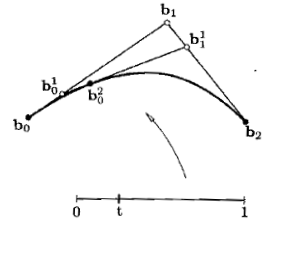
\includegraphics[width=8cm]{../png/repeatedlinear}}
\caption{Construction of a quadratic Bezier spline, taken from ref~\cite{farin}.
The point on the curve parameterised by~$t$ is produced by splitting each of the
lines $b_0 b_1$ and~$b_1 b_2$ in the ratio $t:(1-t)$, then splitting the
line joining the new points in the same proportion.
\label{fig:repeatedlinear}}
\end{figure}

NURBS are preferred because of their greater flexibility
in the ability to generate smooth surfaces.
The flexibility comes at a price however, which may be
paid when two quite distinct NURBS surfaces need to be joined, so-called
`trimmed NURBS'. There are no
simple mathematical formulae to determine NURBS surface intersection, and so recourse
has to be made to some kind of approximation. In practice what may be done
is to consider the intersection curve as the definitive, independent 3-D object.
This however will not lie exactly on either NURBS surface, each of which becomes
more of a guide than a definition of where the surface lies as the bounding
curves are approached. Alternatively the trim curves may be defined in terms of
the surface parameters, either as short line segments or as parametric NURBS, but then
each surface at the join will have a slightly different `intersection' curve.

\begin{figure}
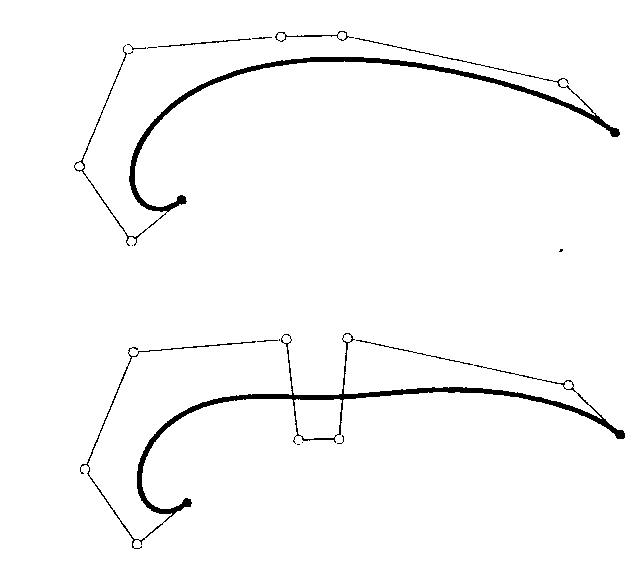
\includegraphics[width=12cm]{../png/pullbezier}
\caption{How CAD is often produced, taken from ref~\cite{farin}.
 The designer moves two of the control points, shown
as open circles, to shape the curve.
\label{fig:pullbezier}}
\end{figure}

Even when topological
information \emph{is} stored such as in the STEP or other proprietary
formats, the use of approximation in surface intersection,
in combination with round-off error, can still lead to the appearance
of small spurious features.
There may be genuine small features in a CAD database, eg.\ small pipework,
rivet heads and other fasteners. For many codes these may not be important
and are undesirable
because by increasing the number of objects to be modelled, they also increase the
code running time. Thus, the first problem to be treated by a CAD interface
is to remove both spurious and genuine small geometrical
features by `CAD repair and defeaturing'. An indication of the size
of this problem is that this was the principal aim of the CADfix$^{TM}$ software
which represents many man-years of development effort. Even with modern
software tools and the results of years of research, to replicate this software
from scratch would be expected to take man-years. Finally at the end
of this process, there is a consistent B-rep ready for meshing.

